\documentclass[12pt,a4paper,utf8]{article} 

\usepackage{abstract} 
\usepackage{amsmath}  
\usepackage{authblk}
\usepackage{array}
\usepackage{appendix}
\usepackage{booktabs} %绘制表格  
\usepackage{biblatex} 
\usepackage{caption2} %标题居中
\usepackage{color} 
\usepackage{colortbl}
\usepackage{ctex}
\usepackage{CJK}
\usepackage{enumerate}  
\usepackage{fancyhdr} 
\usepackage{float}
\usepackage{fontspec} 
\usepackage[marginal]{footmisc}
\usepackage{geometry} 
\usepackage{graphicx}  
\usepackage[hidelinks]{hyperref}
\usepackage{lastpage}
\usepackage{listings} 
\usepackage{longtable} 
\usepackage{minted}
\usepackage{multirow}
\usepackage{biblatex}
\usepackage{subfigure}
\usepackage{soul}
\usepackage[svgnames]{xcolor}
\usepackage[table]{xcolor}
\usepackage{titlesec} 
\usepackage{type1cm}
\usepackage{times}


\newcommand*{\arraycolor}[1]{\protect\leavevmode\color{#1}}
\newcolumntype{A}{>{\columncolor{blue!50!white}}c}
\newcolumntype{B}{>{\columncolor{LightGoldenrod}}c}
\newcolumntype{C}{>{\columncolor{FireBrick!50}}c}
\newcolumntype{D}{>{\columncolor{Gray!42}}c} 

\geometry{a4paper, left=2.5cm, right=2.5cm, top=2.5cm,bottom=2.5cm}%设置页面尺寸
\lstset{
		numbers=left, %设置行号位置
		numberstyle=\tiny, %设置行号大小
		keywordstyle=\color{blue}, %设置关键字颜色
		commentstyle=\color[cmyk]{1, 0, 1, 0}, %设置注释颜色
		escapeinside=``, %逃逸字符(1左面的键), 用于显示中文
		breaklines, %自动折行
		extendedchars=false, %解决代码跨页时, 章节标题, 页眉等汉字不显示的问题
		xleftmargin=1em, xrightmargin=1em, aboveskip=1em, %设置边距
		tabsize=4, %设置tab空格数
		showspaces=false %不显示空格
}

\pagestyle{fancy}
% 页眉设置  
\fancyhead[L]{}
\fancyhead[C]{基于电影《雄狮少年》的网络舆情分析大数据报告}
\fancyhead[R]{}
% 页脚设置
\fancyfoot[C]{Page \thepage\ of \pageref{LastPage}} % 页码
\renewcommand{\headrulewidth}{2pt} % 分隔线宽度2磅
% \renewcommand{\footrulewidth}{1pt}
 
   
\title{\HUGE{\textbf{基于电影《雄狮少年》的舆情分析大数据报告}}}
\author[1]{王红阳}
\author[2]{夏睿} 
\author[3]{周浩然}
\author[4]{窦浩阳}

\affil[1]{天津大学智能与计算学部-3019244233}
\affil[2]{天津大学智能与计算学部-3019244105} 
\affil[3]{天津大学智能与计算学部-3019244229} 
\affil[4]{天津大学智能与计算学部-3019202235} 
\renewcommand*{\Affilfont}{\small\it} % 修改机构名称的字体与大小
\date{} % 去掉日期


\begin{document}
\pagenumbering{Roman} %设置罗马数字页码

\begin{figure}[t]
\centering
	
\includegraphics[scale=0.4]{images/图标.png} 
\end{figure}

\maketitle % 显示标题
 
\phantomsection\addcontentsline{toc}{section}{摘要}\tolerance=500
\begin{abstract} 
在信息发展多元化的今天,网络舆情对我国的社会生活产生了越来越深远的影响。\\

在近期,动漫电影《雄狮少年》引起了人们的激烈讨论,一方说其为辱华动漫,一方对其赞赏有加。我们选取它作为研究对象,使用各种舆情分析方式,还原公共视角。我们使用Python爬虫抓取各社交平台的约5万条用户发言,使用中文分词处理、词频统计和贝叶斯法则等方法,进行话题挖掘和情感计算,以对这一现象进行舆情分析。用词频统计和贝叶斯情感值计算来显示民众的看法和想法,然后使用TF-IDF计算、LDA话题模型,回归分析及K-means聚类方法来挖掘群众观点。结果显示,各社交平台对其看法差异较大,存在割裂现象,侧面印证了我国互联网的回声室效应。\\

 
 \textbf{[Key Words]}:  网络舆情分析、大数据、雄狮少年、社交媒体、可视化

\end{abstract}

\setcounter{page}{1}
\thispagestyle{empty} % 取消页脚

\newpage %分页
\pagenumbering{arabic} %设置数字页码

\thispagestyle{empty} % 取消页脚
% 目录
\renewcommand{\contentsname}{\centerline{目 \quad 录}}
\begin{center}
    \tableofcontents
\end{center}

\thispagestyle{empty} % 取消页脚


\newpage  
\section{背景及意义}
随着大数据时代的到来,数据从简单的处理对象开始转变为一种基础性资源。而随着互联网的不断普及,越来越多网民选择利用社交网络展现其对于现实世界的关注,藉由网络表达自身意见、宣泄自身情绪,互联网平台逐渐成为现实事件发展的传感器,而网络舆情也在反映民意、折射现实中承担着越来越重要的作用。 \\

如何利用计算机方法和情感挖掘方法来准确识别民众的情绪状态和倾向,已经成为一个重要的问题。 \\ 

在线社交网站为人们提供了一个构建社会关系网络和互动的平台。每一个人和组织都可以通过社交网站互动、获取信息并发出自己的声音,因而吸引了众多的使用者。作为一个复杂的社会系统,在线社交网站真实地记录了社会网络的增长以及人类传播行为演化。通过抓取并分析在线社交网站的数据,我们可以迅速地把握人类社交网络行为背后所隐藏的规律。\\

本文充分利用大数据技术和人工智能技术,从各社交平台挖掘热点舆情话题,从网民对该话题所发表的图、文、声、像等多媒体意见的分析中挖掘提炼对观点、情感和态度,进行舆情分析。 \\

我们观察到,在近期,有一部动漫电影引起了人们的激烈争论,它就是《雄狮少年》。我们选取它作为我们的网络舆情研究对象。\\
 
为此, 我们使用Python爬虫抓取各社交平台的约5万条用户发言,使用中文分词处理、词频统计和贝叶斯法则等方法,进行话题挖掘和情感计算,以对这一现象进行舆情分析。 \\

用词频统计和贝叶斯情感值计算来显示民众的看法和想法,然后使用TF-IDF计算、LDA话题模型,回归分析及K-means聚类方法来挖掘在这一问题上的群众观点。

\section{技术路线}
\begin{figure}[H]
    \centering
    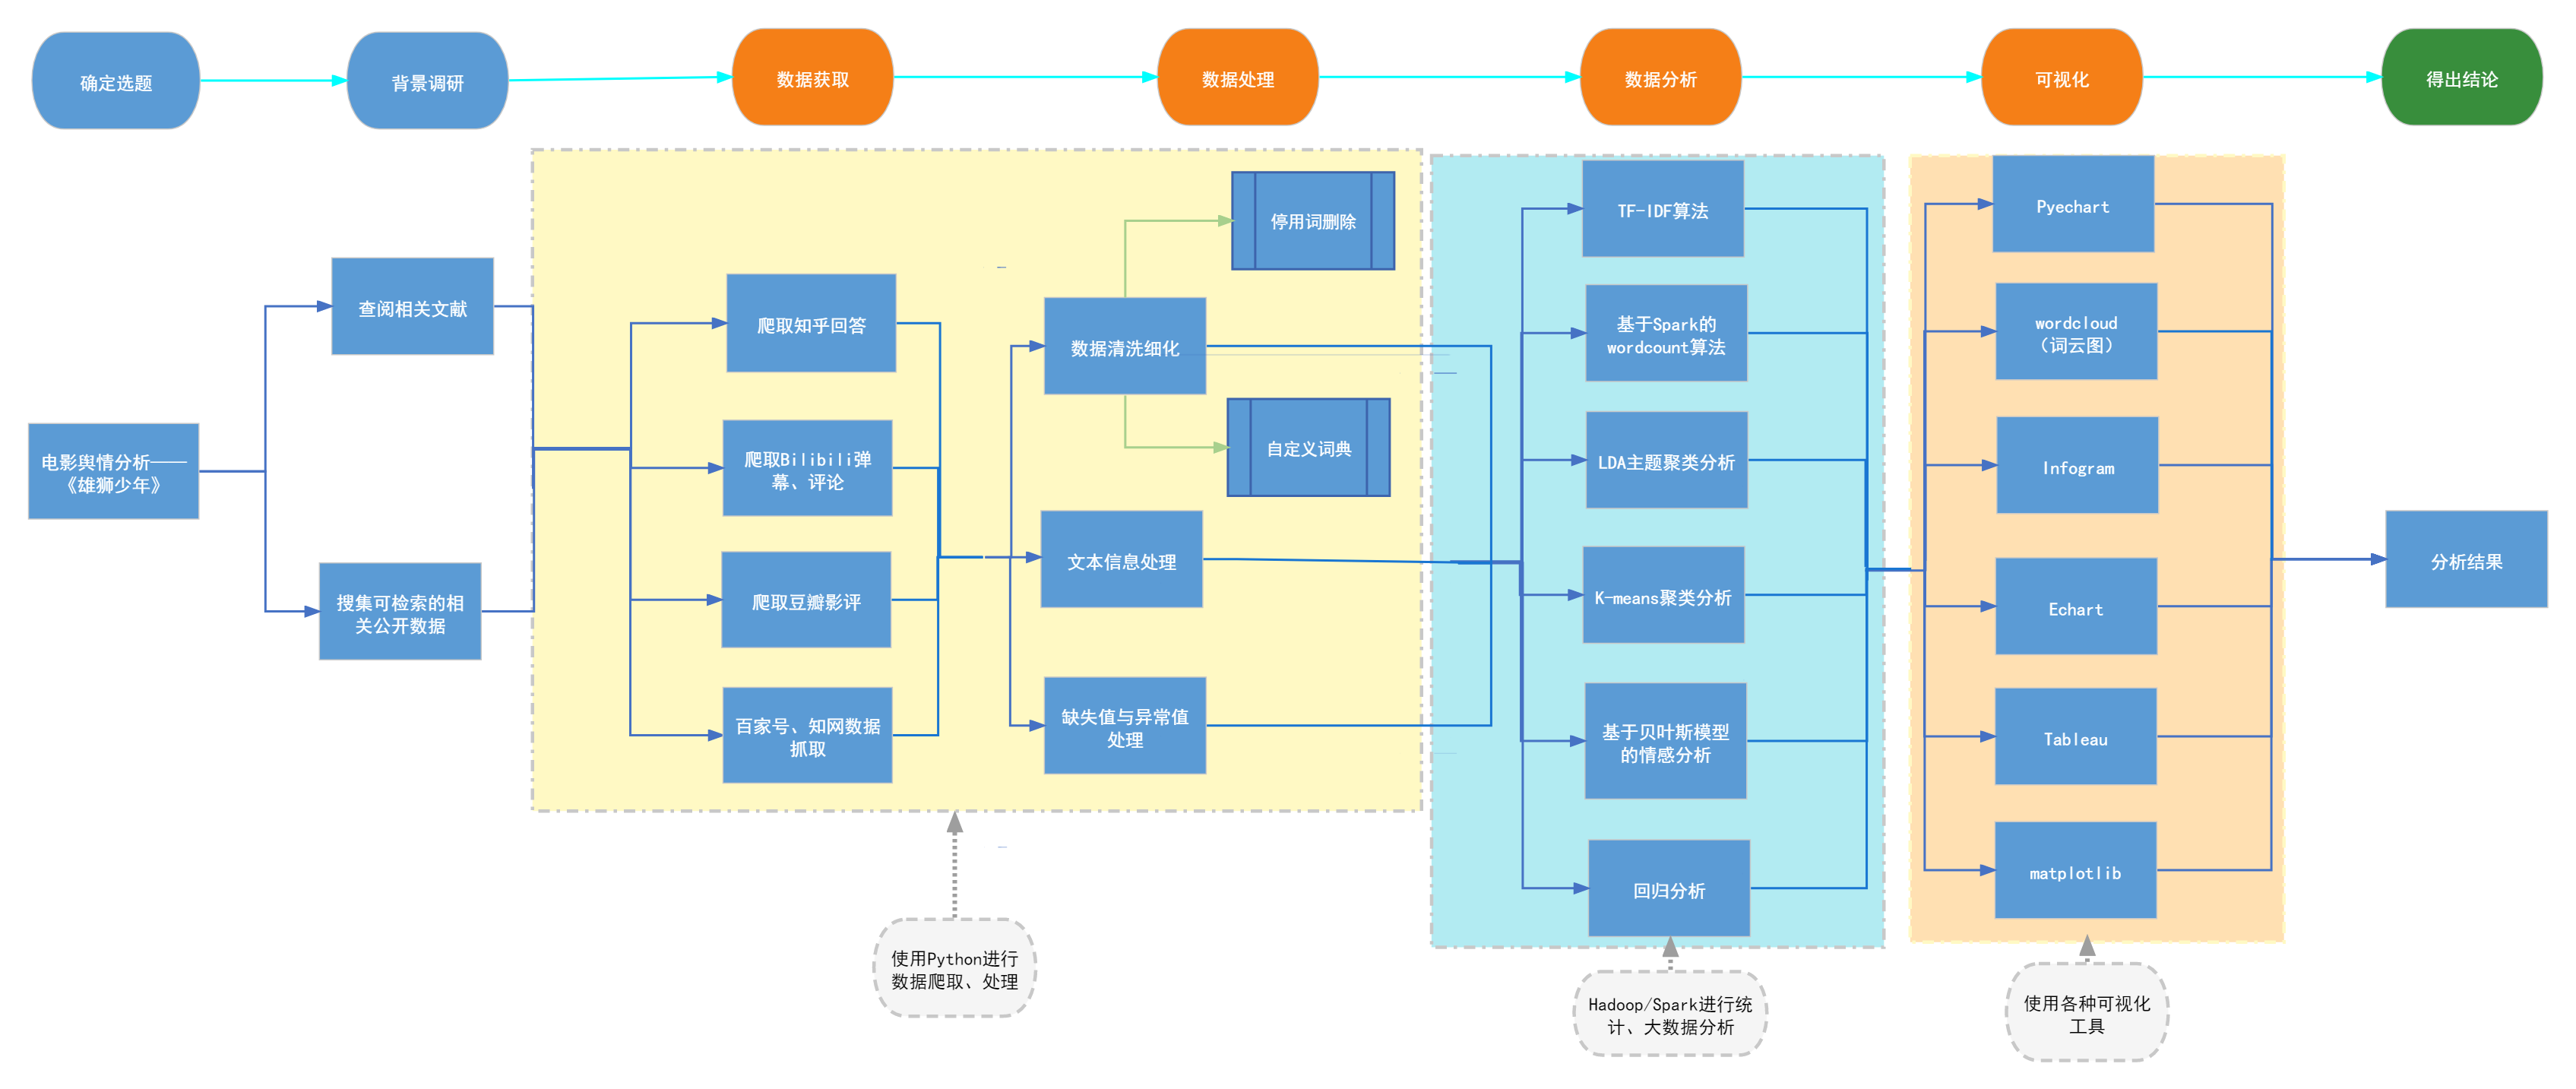
\includegraphics[width=1\textwidth]{images/技术路线.png}  
    \caption{技术路线图} 
\end{figure}  

上图为我们的技术路线图\footnote{\color{red}{建议放大查看}}。\\

我们在社交类、知识分享类、娱乐类的热门平台,使用python爬虫爬取涉及该电影及该话题的数据,数据格式包括问题回答,弹幕,短评,文章等。 \\

在此基础上,经过数据清洗和预处理,将获取到的数据,分别用于以下几个方面:
\begin{enumerate}
\item 豆瓣影评分析:词云图生成,K-means聚类分析,回归分析;
\item 知乎回答分析:LDA主题聚类、情绪分类等;
\item bilibili视频弹幕及评论:词云图生成;
\end{enumerate}  

\section{数据采集}

\subsection{前期工作}
舆情分析,最关键的就是时效性。为此,我们首先根据百度搜索指数,确定我们所需爬的数据的时间范围,避免爬取过时数据。\\ 

由该搜索指数图,可以得知,为了分析大家对于电影《雄狮少年》的舆情变化,我们需要爬取的数据时间范围大约为:2021年的12月至2022年的1月。

\begin{figure}[H]
    \centering
    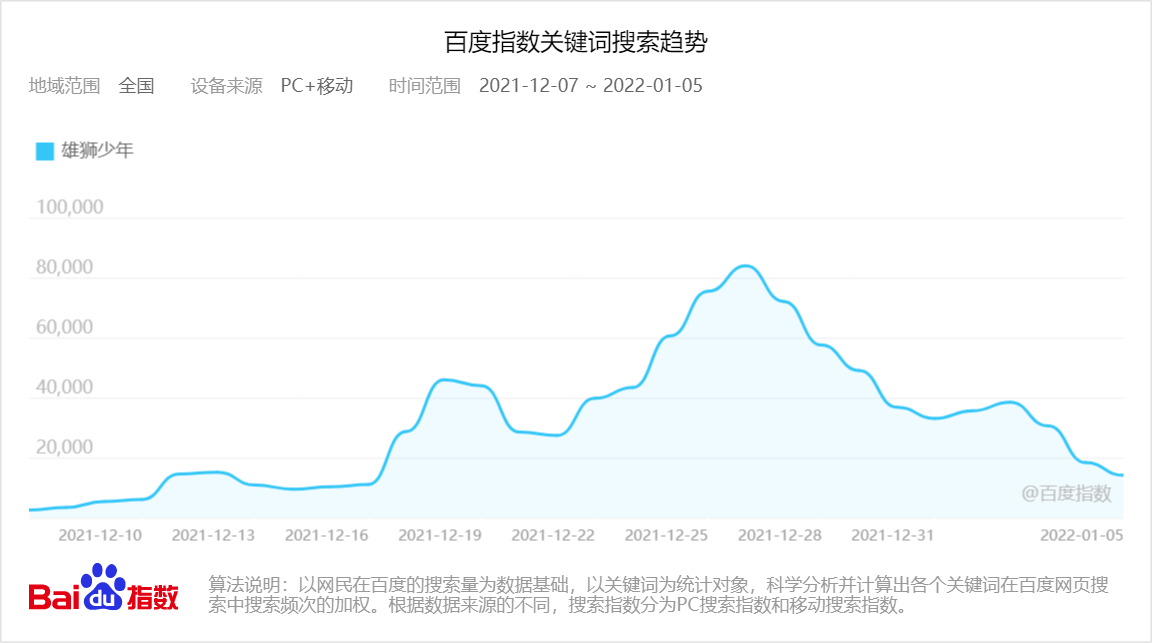
\includegraphics[width=0.9\textwidth]{images/百度指数.png}  
    \caption{雄狮少年搜索指数} 
\end{figure}  

其次,电影《雄狮少年》的相关搜索词,也是一个重要的地方,我们可以根据它,扩充索索关键词,以爬取更多数据用于分析。
\begin{figure}[H]
    \centering
    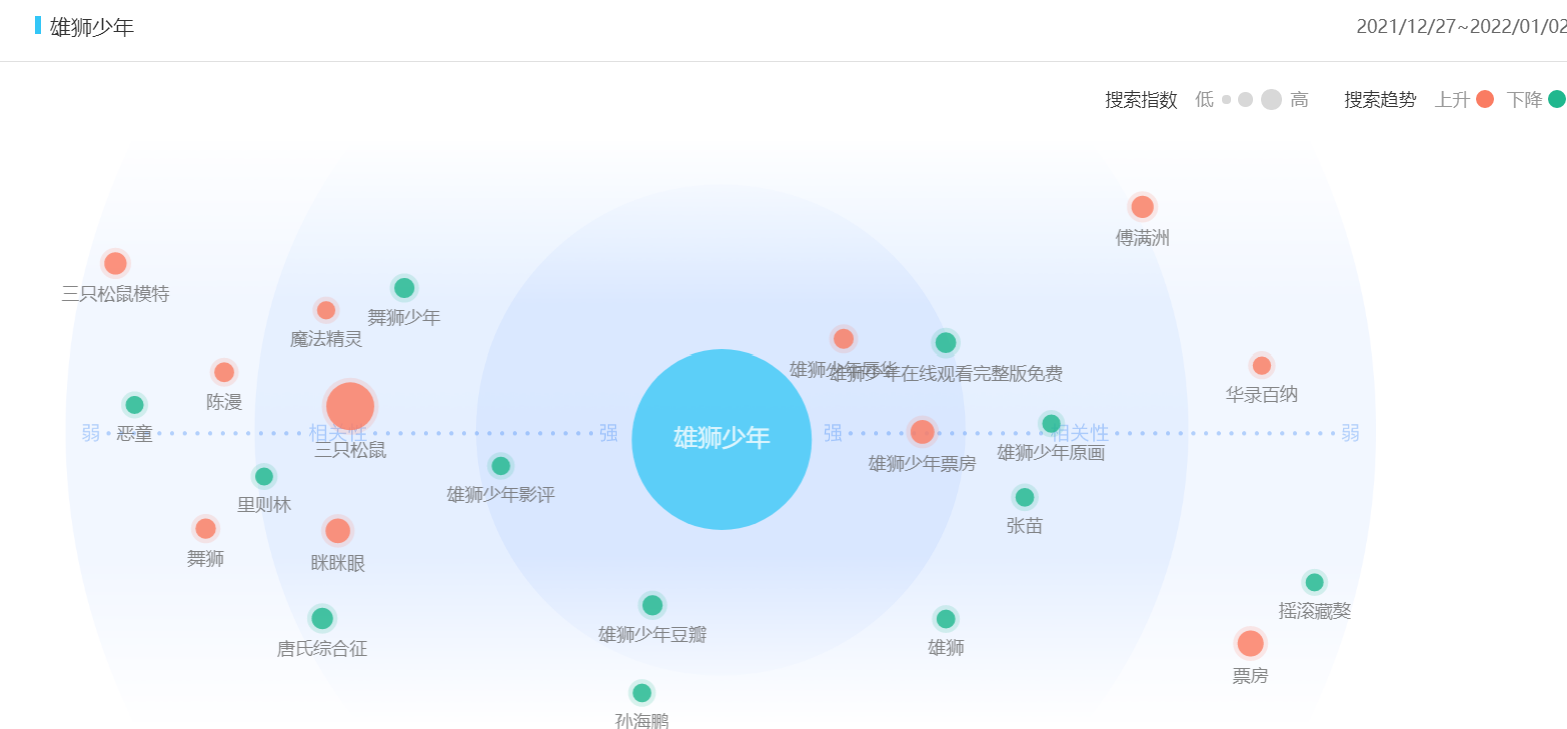
\includegraphics[width=0.9\textwidth]{images/相关搜索.png}  
    \caption{雄狮少年相关搜索} 
\end{figure}  

确定时间和爬取关键词后,我们还需确定频繁在该问题下发言的人处于什么年龄阶段,以确定爬取哪些平台的数据(不同平台有不同年龄的受众)
\begin{figure}[H]
    \centering
    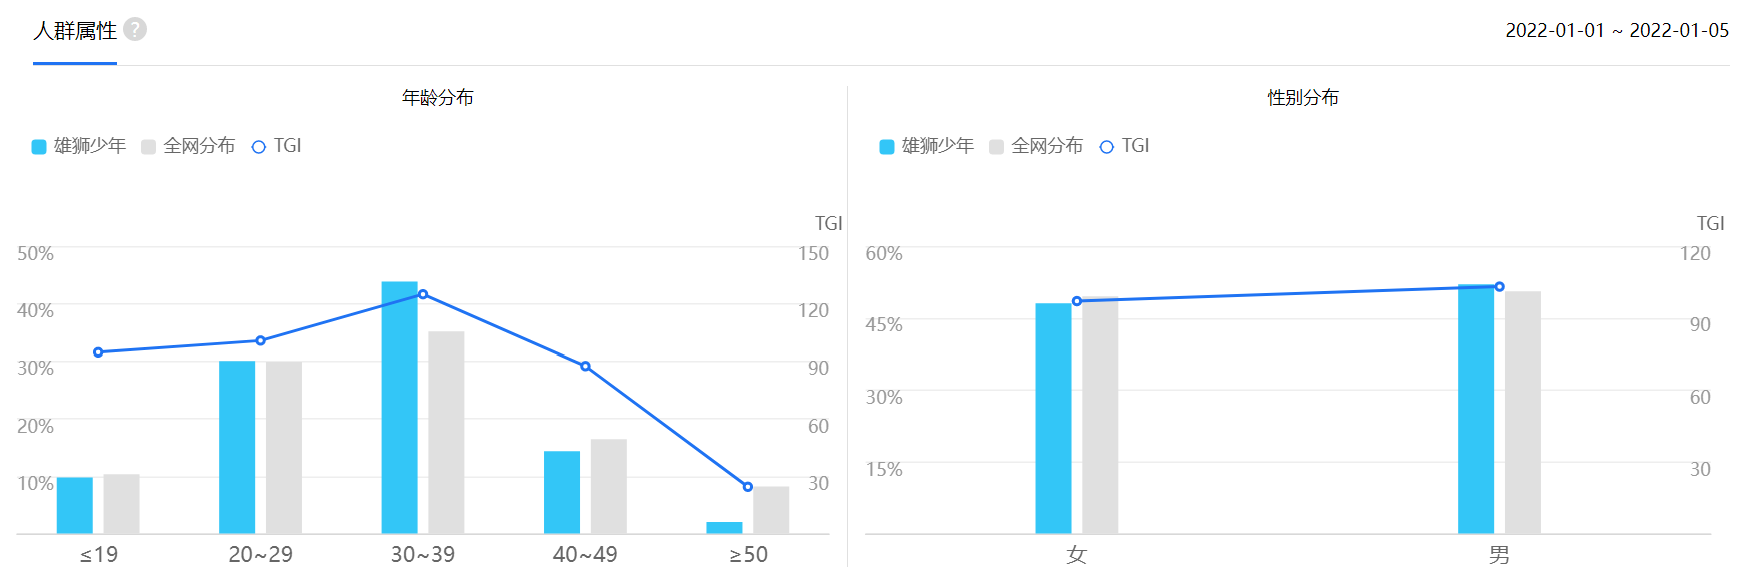
\includegraphics[width=1\textwidth]{images/人群属性.png}  
    \caption{近期关注该问题的人群属性} 
\end{figure}  
关注该问题的人群中,男女比例男性偏多,几乎相等,以年轻人和中青年偏多。这给我们的数据爬取带来很大帮助,因为他们在社交平台上发言更频繁,更容易获取来及他们的讨论。为此,我们选取了受年轻人青睐的以bilibili弹幕网,知乎网和豆瓣网为主的社交平台,来进行舆情分析。

\subsection{百家号}
百家号是百度为内容创作者提供的内容发布、内容变现和粉丝管理平台;提供百亿级流量致力于让内容恰如其分地找到读者。\\

使用八爪鱼采集器抓取百家号平台里,所有关键词为雄狮少年的文章共400余条,涉及时间范围为:2021.12.28-2022-01-06,具体内容包括关键词,页面网址,标题,正文,博主,发布时间,博主账号等

\subsection{豆瓣}
豆瓣网是国内影迷最为重要的电影交流阵地。大量具有较高互动频度的影迷聚集在一起,成为国产电影的重要舆论场。其影片评分为影片整体的舆论做出定位,成为社会公众观影选择的参照系。 \\

我们使用Python爬取来自对于电影《雄狮少年》的影评约4000条.

\begin{figure}[H]
    \centering
    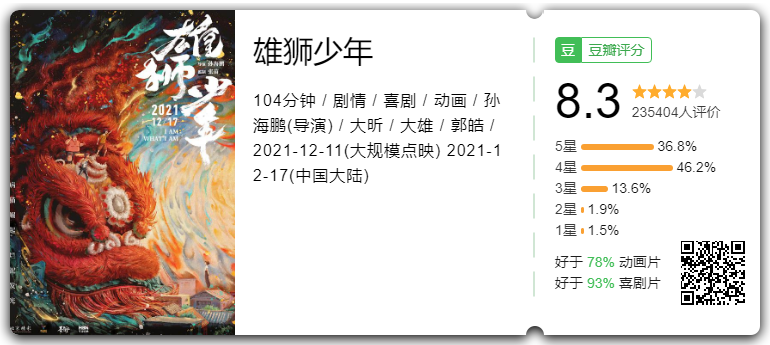
\includegraphics[width=0.6\textwidth]{images/雄狮少年.png}  
    \caption{电影《雄狮少年》} 
\end{figure} 


\subsection{知乎}
知乎是一个中文互联网高质量的问答社区和创作者聚集的原创内容平台。\\
 
我们使用Python爬虫,爬取来自关于本电影的问题下的全部回答,约10000条 \\
\begin{figure}[H]
    \centering
    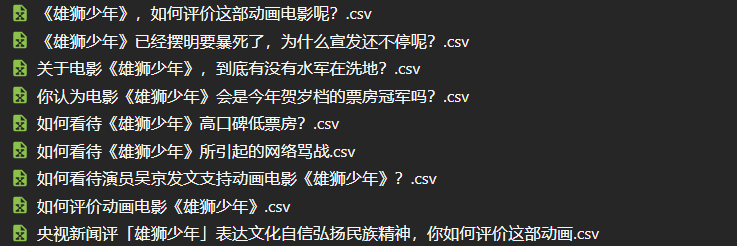
\includegraphics[width=0.6\textwidth]{images/知乎问题.png}  
    \caption{知乎热门问题} 
\end{figure} 


\begin{table}[H]   
\sffamily
\arrayrulecolor{white}
\arrayrulewidth=1pt
\renewcommand{\arraystretch}{1.5}
    \begin{tabular}{A||B|C|A|B|C|A} 
    \rowcolor{.!80!Black}
     \arraycolor{White}\bfseries 代码变量 &  author &  fans\_count & content & created\_time  & comment\_count & voteup\_count \\
     \hline
     \arraycolor{White}\bfseries 实际意义 & 作者昵称  & 粉丝数   & 回答正文 & 回答创建时间 &  回答评论数  &  回答赞成数 \\ 
    \end{tabular}
    \caption{知乎回答格式} 
\end{table}
 

如下图所示:


\begin{figure}[H]
    \centering
    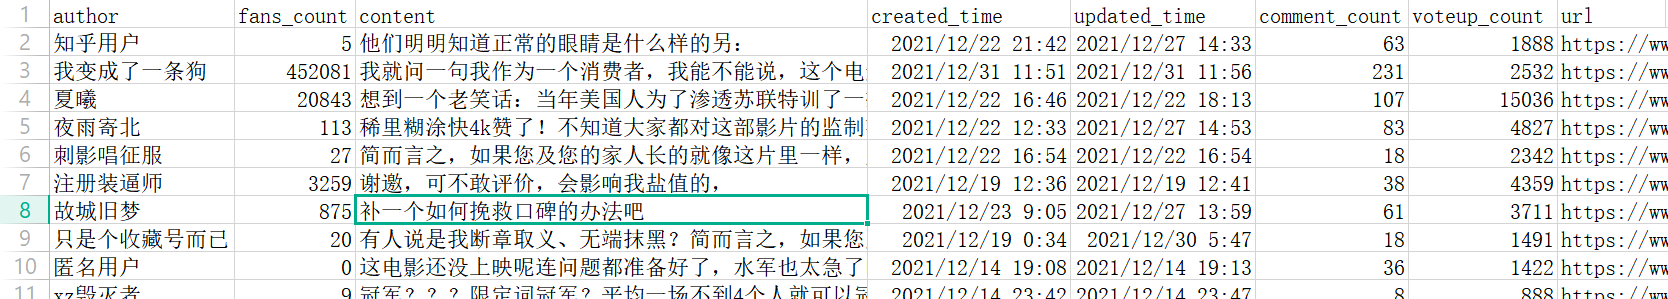
\includegraphics[width=1\textwidth]{images/知乎问题信息.png}  
    \caption{知乎回答数据格式} 
\end{figure}  

\subsection{bilibili}
bilibili是国内知名的视频弹幕网站,我们爬取涉及本电影的视频的弹幕及评论,约4万条 \\

\begin{table}[H]  
\begin{center}
\sffamily
\arrayrulecolor{white}
\arrayrulewidth=1pt
\renewcommand{\arraystretch}{1.5}
    \begin{tabular}{A||B|C|A|B|C|A|B} 
    \rowcolor{.!80!Black}
     \arraycolor{White}\bfseries 代码变量 &   username & sex & level & content & replies\_num & like & voteup\_count \\
     \hline
     \arraycolor{White}\bfseries 实际意义  & 用户昵称 & 性别 & 等级  & 回答内容 & 评论回复数 & 评论获赞数 & 回答赞成数 \\
    \end{tabular}
    \caption{视频弹幕数据格式} 
\end{center}
\end{table}  


\subsection{知网}
知网即中国知网,又被称为“中国期刊网”,是中国最大的学术论文数据库和学术电子资源集成商。\\

在中国,知网可以用一家独大来形容其在数据库集成商中的地位。

我们使用八爪鱼采集器了来自知网的相关论文信息,但由于知网的学术性质,不适合做时效性较强的舆情分析,故获得的数据不多,仅有10条,故不适合用于舆情分析。 \\

\subsection{数据统计}
我们对数据进行了去重、去空操作,并调整了数据的编码格式。最终数据占比图,如下:
\begin{figure}[H]
    \centering
    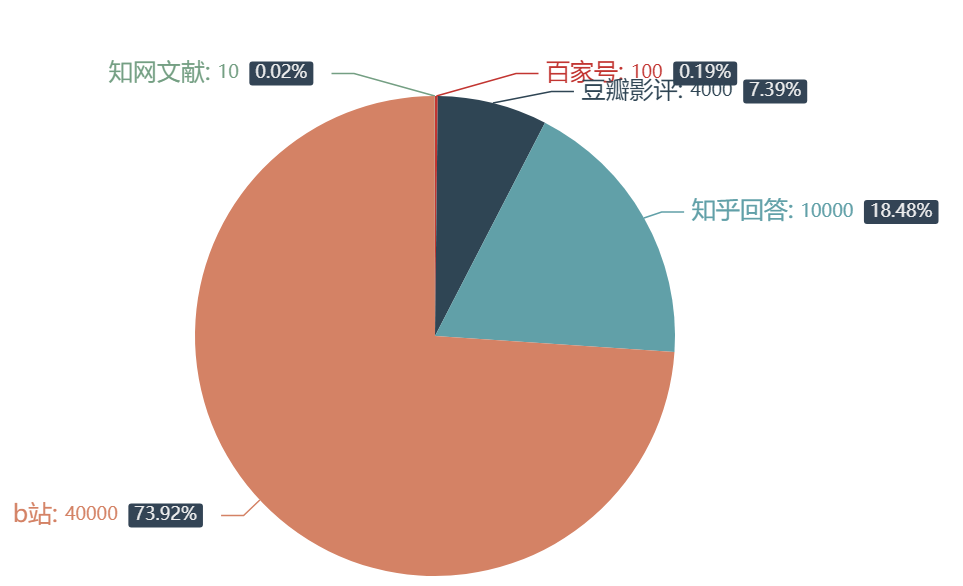
\includegraphics[width=0.7\textwidth]{images/数据量占比.png}  
    \caption{数据量占比} 
\end{figure}   


\section{基于大数据算法的数据可视化分析}
\subsection{基于wordcount的词云图分析}
我们设计了基于 spark 的 wordcount算法用于分析评论中的词频统计。

\subsubsection{流程及代码}
基于 spark 的 wordcount 算法流程图如下:
\begin{figure}[H]
    \centering
    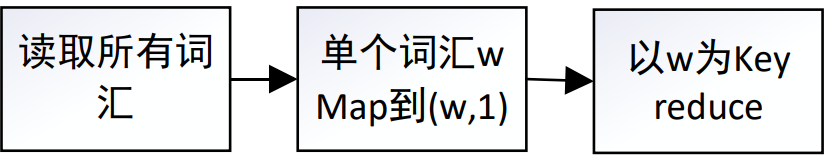
\includegraphics[width=0.6\textwidth]{images/wordcount.png}  
    \caption{wordcount流程图} 
\end{figure}  
核心代码为:
 
\begin{minted}[linenos, numbersep=5pt, frame=lines, framesep=2mm, autogobble]{Python} 
data.flatMap(lambda x:.split(' ')).map(lambda x:(x,1)).reduceByKey(lambda a,b:a + b)
\end{minted}   

得到词频统计后,在此之上可以画出词云图,以得到人们的发言关键词,也可按照词汇的正负性等进行进一步的细粒度划分。 \\

\subsubsection{词云可视化及分析}
利用得到的词频,制作词云图进行可视化展示。
\begin{figure}[H]
\centering
\subfigure 
{  
    \begin{minipage}[b]{.45\textwidth}
        \centering 
        \caption{豆瓣词云图}
        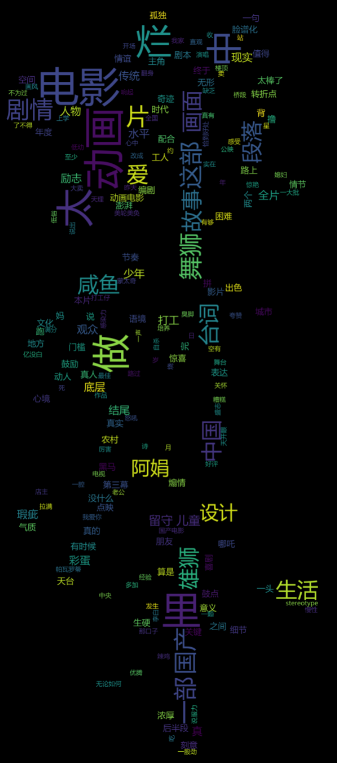
\includegraphics[width=0.6\textwidth]{images/douban.png}
     \end{minipage}
}
\subfigure 
{  
    \begin{minipage}[b]{.45\textwidth}
        \centering
        \caption{知乎词云图}
        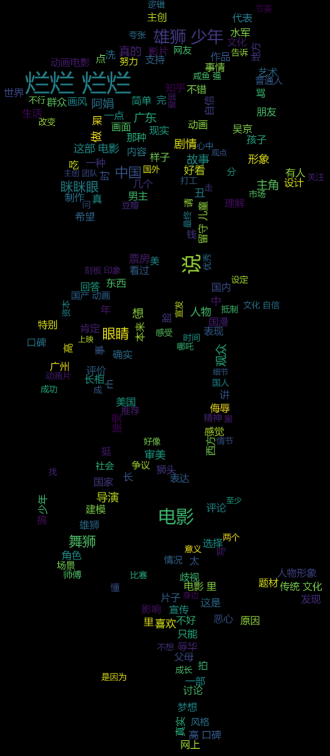
\includegraphics[width=0.6\textwidth]{images/zhihu.png}
    \end{minipage}
     
} 
\end{figure} 
如图,我们可以看到在知乎词云图中,出现了更多负面词汇:烂、眯眯眼\footnote{西方人在嘲笑中国人的时候,常常会做这样一个动作:就是双手把眼角往上拉,形成俗称的“眯眯眼”。这代表了西方人对中国人的一种刻板的印象,通常会被做视为辱华的象征}、水军、歧视等词汇。

\begin{figure}[H]
    \centering
    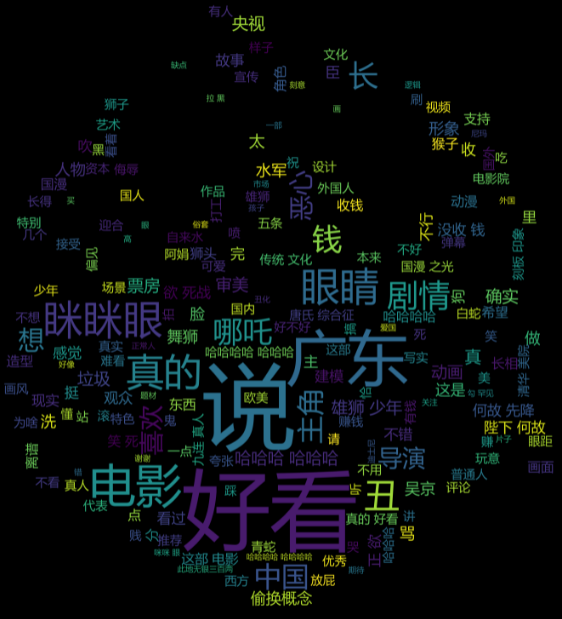
\includegraphics[width=0.5\textwidth]{images/bilibili.png}  
    \caption{bilibili视频弹幕词云图} 
\end{figure}  
视频弹幕,更为口语化,该词云图里面几乎全是贬义词,这也说明了,年轻人很可能并不喜欢这部电影。


\subsection{TF-IDF算法}
TF-IDF有两层意思,一层是"词频"(Term Frequency,缩写为TF),另一层是"逆文档频率"(Inverse Document Frequency,缩写为IDF)。 \\ 

当有TF(词频)和IDF(逆文档频率)后,将这两个词相乘,就能得到一个词的TF-IDF的值。某个词在文章中的TF-IDF越大,那么一般而言这个词在这篇文章的重要性会越高,所以通过计算文章中各个词的TF-IDF,由大到小排序,排在最前面的几个词,就是该文章的关键词。 \\

获取每篇文章的关键词之后,我们可以去做LDA主题聚类,以确定这些文章各自所属的主题。

\subsection{LDA主题聚类分析}

\subsubsection{算法原理}
我们设计了基于 spark 实现的 LDA 算法,LDA 是一种经典的主题模型,常用于文本分
类任务。该模型是包含词、主题、文档在内的三层贝叶斯概率模型,该模型使用词袋模型,将每篇文档视为一个词频向量,从而得到文档到主题的多项式分布和主题到词的多项式分布。
\begin{figure}[H]
    \centering
    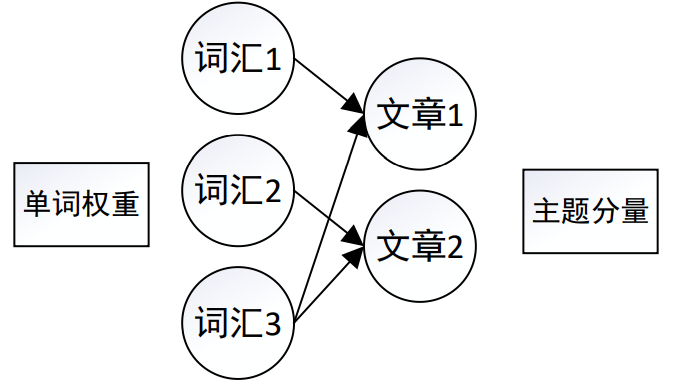
\includegraphics[width=0.6\textwidth]{images/LDA.png}  
    \caption{LDA原理图} 
\end{figure}  
LDA适合长文本,因此我们选用知乎回答,来进行数据分析。
对于我们的任务而言,我们希望对该电影的知乎回答来进行聚类,尝试对其主题进行分析。因此,我们借助spark中的lda模型实现了文本主题聚类算法。\\

具体地,首先读取存储在csv文件中的知乎回答数据,接着,对读取的数据进行分词、去除停用词等常规预处理操作,生成 RDD 后调用 LDA 模型进行无监督的聚类,流程图如下:
\\
\begin{figure}[H]
    \centering
    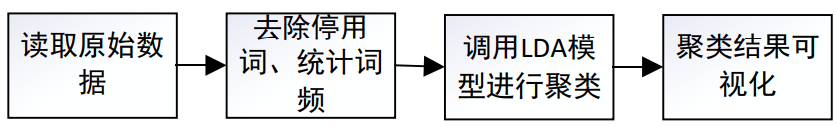
\includegraphics[width=0.8\textwidth]{images/LDA流程.png}  
    \caption{LDA流程图} 
\end{figure}  

\subsubsection{核心代码}

\small{
\begin{minted}[linenos, numbersep=5pt, frame=lines, framesep=2mm, autogobble]{Python} 

text_data = spark.read.format("csv").option("header",True).load("/usr/local/all.csv")

# 分词
tokenizer = ft.RegexTokenizer(inputCol='documents',\
            outputCol='input_arr',pattern=r'\s+|[,.\"]')

# 去停用词
stopwords = ft.StopWordRemover(inputCol=tokenizer.getOutputCol(),outputCol='input_stop')

# 统计词频
stringIndex = ft.CountVectorizer(inputCol=stopwords.getOutputCol(),\     
                outputCol='input_indexed')

clustering = clus.LDA(k=5,optimizer='online',featuresCol=stringIndex.getOutputCol())

\end{minted}}

\subsubsection{数据可视化及分析}
得到的各个主题及词频如下:

\small{ 
$\bullet$ 主题0:
 
0.015*"电影" + 0.015*"雄狮" + 0.010*"说" + 0.009*"故事" + 0.008*"舞狮" + 0.008*"没有" + ... \\

$\bullet$ 主题1: 

0.029*"说" + 0.018*"电影" + 0.013*"觉得" + 0.012*"眼睛" + 0.010*"没" + 0.008*"眯眯眼" + ...  \\

$\bullet$主题2:

0.014*"舞狮" + 0.006*"雄狮" + 0.006*"没有" + 0.005*"说" + 0.005*"电影" + 0.005*"会" + ... \\

$\bullet$ 主题3: 

0.019*"票房" + 0.017*"雄狮" + 0.015*"电影" + 0.013*"中国" + 0.009*"口碑" + 0.009*"没有" + ...  \\

$\bullet$主题4: 

0.019*"电影" + 0.012*"说" + 0.011*"文化" + 0.010*"会" + 0.009*"中国" + 0.008*"没有" + ...  \\
}
   
\begin{figure}[H]
    \centering
    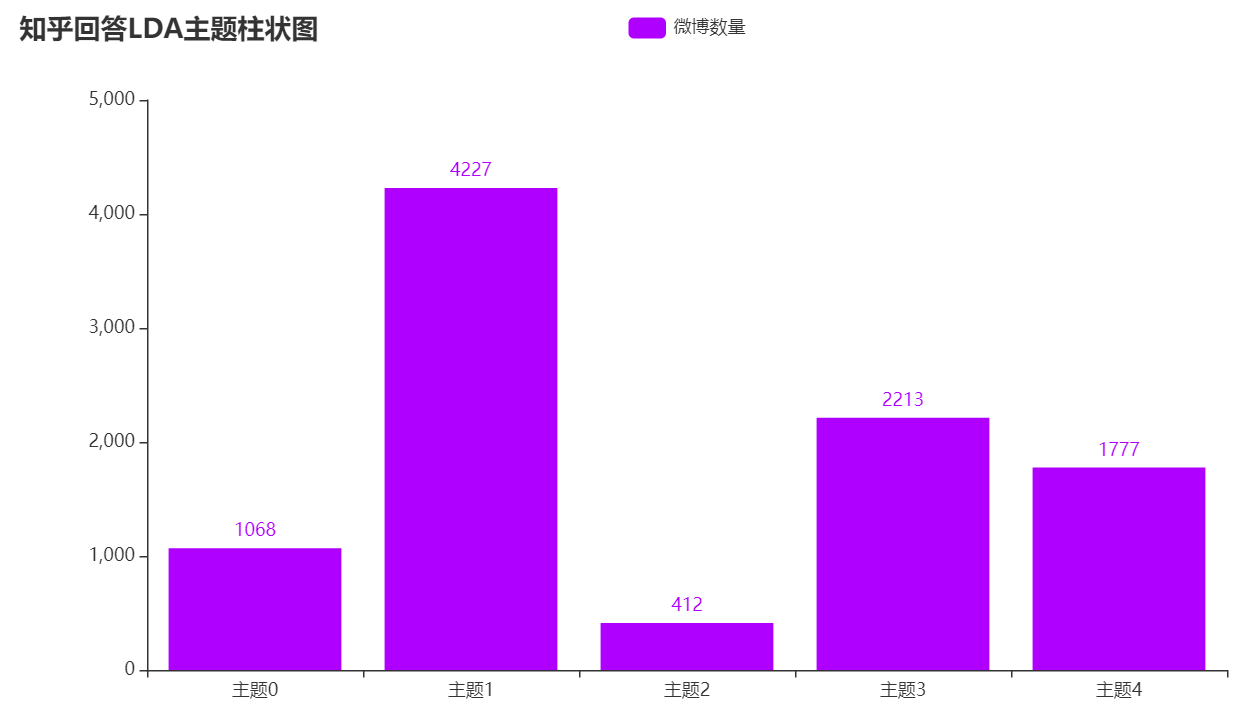
\includegraphics[width=0.7\textwidth]{images/知乎LDA.png}  
    \caption{LDA主题图} 
\end{figure}   

\begin{figure}[H]
    \centering
    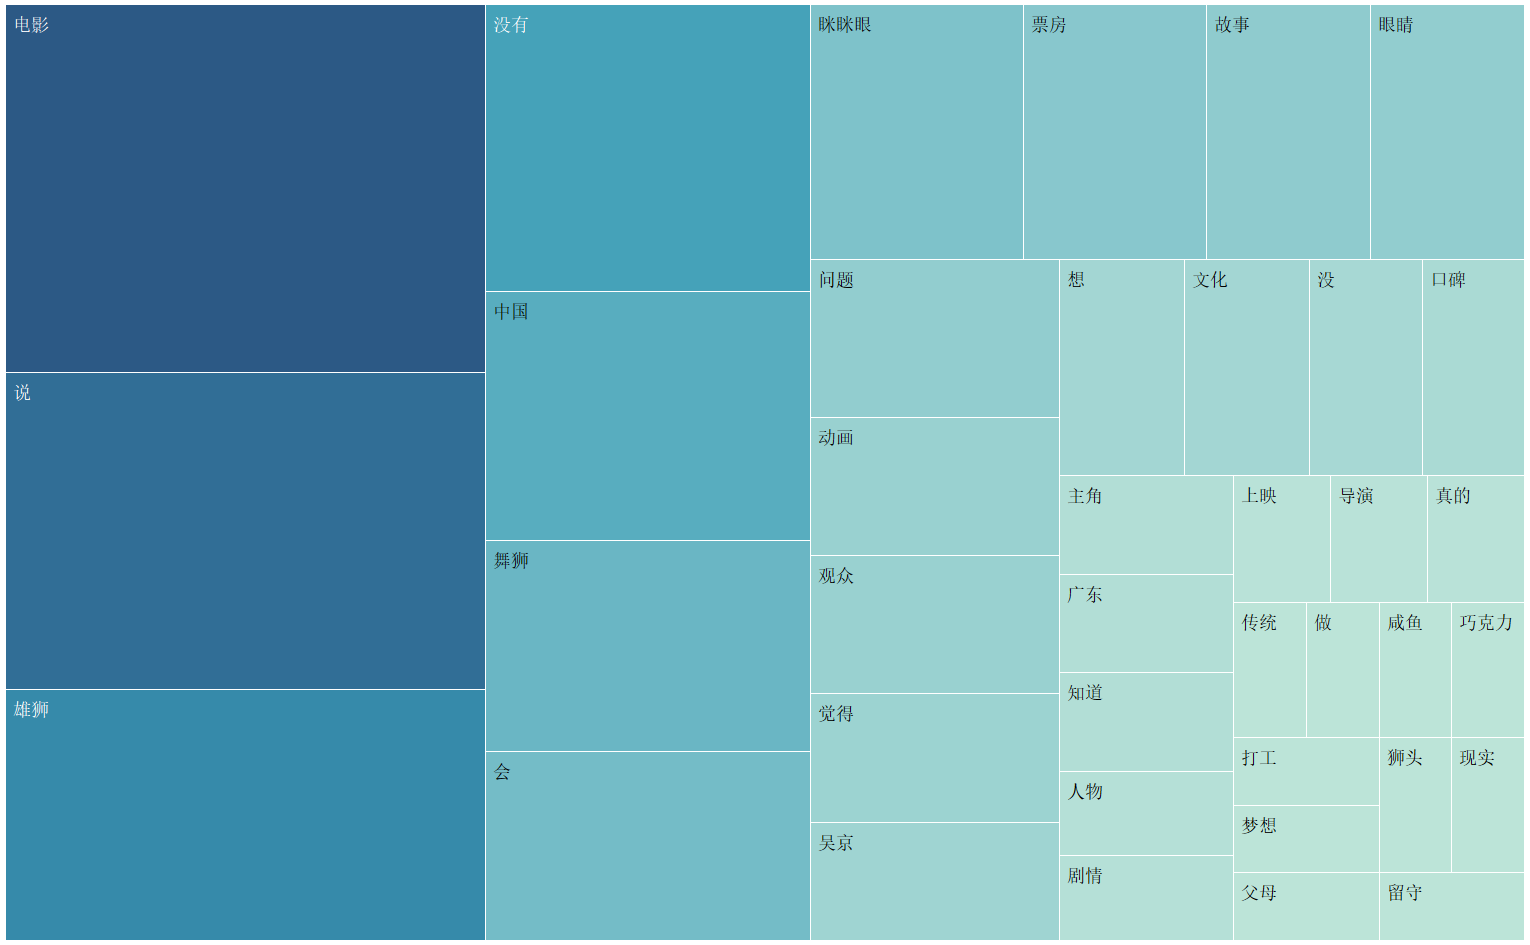
\includegraphics[width=0.9\textwidth]{images/LDA词频图.png}  
    \caption{LDA主题词频}
\end{figure} 

根据各主题关键词的词频以及各主题的文章数目,公众观点主要聚焦到这一电影的票房,这一电影的主题:舞、,广东文化,以及是否存在眯眯眼的辱华现象。

这也侧面说明了该电影可能在在是否辱华这一问题上敏感地触动了公众情绪。

\subsection{情感分析}
我们对该电影的评论进行情感分析,得出对于电影《雄狮少年》的负面评价大于正面评价,这也符合我们从词云图得到的结论。
\begin{figure}[H]
    \centering
    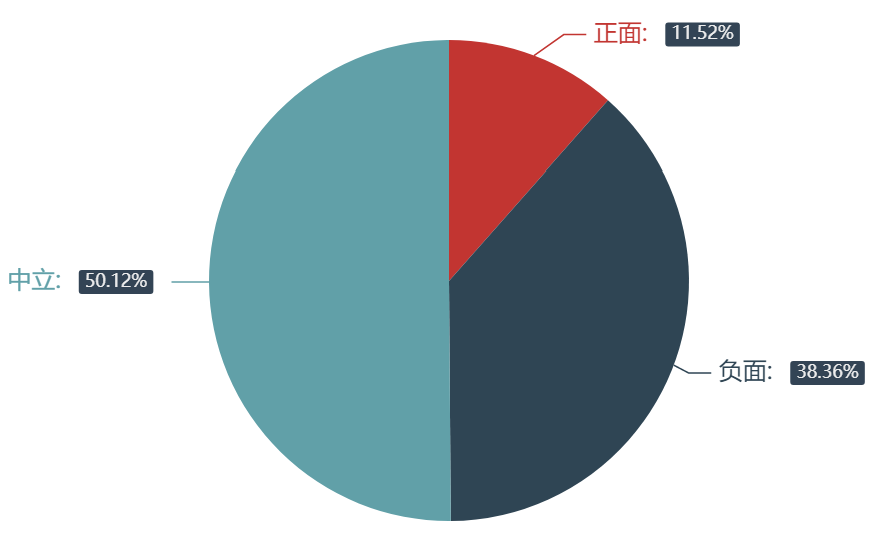
\includegraphics[width=0.6\textwidth]{images/情感倾向.png}  
    \caption{情感倾向图} 
\end{figure}   

 
\begin{table}[H]  
\begin{center}
\sffamily
\arrayrulecolor{white}
\arrayrulewidth=1pt
\renewcommand{\arraystretch}{1.5}
    \begin{tabular}{A|C} 
    \rowcolor{.!80!Black}
    \arraycolor{White}\bfseries 公众情感态度 & 观点列举 \\
    \hline
     \arraycolor{White}\bfseries 正向 & 热血国漫;感受魅力;岭南文化;小镇青年的奇迹 \\
     \hline
     \arraycolor{White}\bfseries 负向 & 很丑;眯眯眼;刻板印象;人设有问题;崇洋媚外 \\
     \hline  
     \arraycolor{White}\bfseries 中立 & 网红审美;艺术处理;角色脸谱鲜明;没有感觉 \\
     \hline
    \end{tabular}
    \caption{公共情感主要示例} 
\end{center}
\end{table}  

我们,可以看到公众情绪并不是那么的激烈,但是显然厌恶这部电影的人数是远远低于喜欢这部电影的人,这将对后续这部电影的票房及影响产生不利影响。


\subsection{k-means聚类分析}
\subsubsection{聚类目标}

豆瓣网用户对《雄狮少年》的星级评分
\begin{figure}[H]
    \centering
    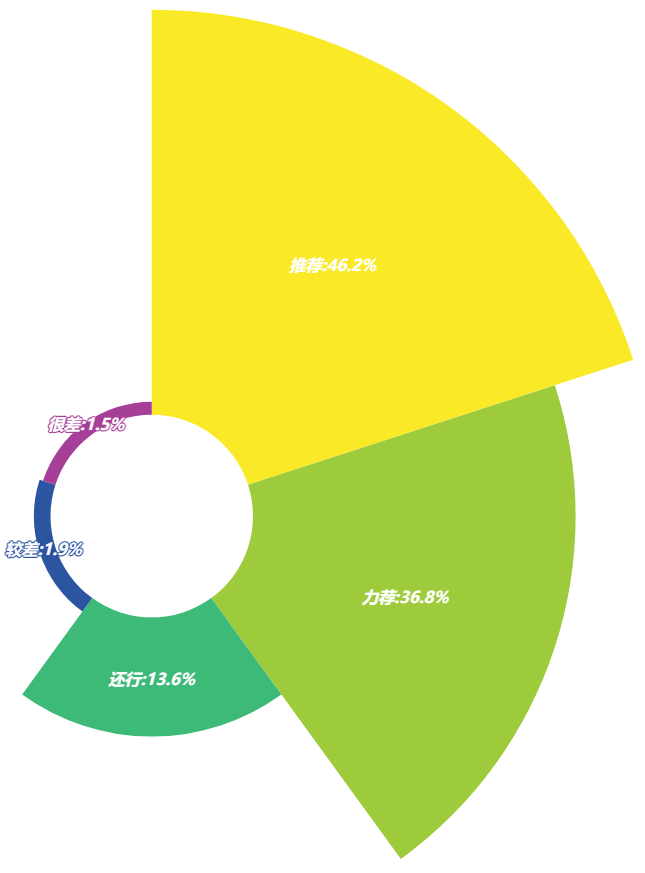
\includegraphics[width=0.4\textwidth]{images/豆瓣评分-.png}  
    \caption{豆瓣评分占比图}
\end{figure}  
 

\subsubsection{核心代码}
\begin{minted}[linenos, numbersep=5pt, frame=lines, framesep=2mm, autogobble]{Python}  
sc = SparkContext(appName="KmeansExample" + file)

# 读入数据
data = sc.textFile(file)
# 数据清洗
parsedData = data.map(lambda line: array([float(x) for x in line.split(' ')]))
# 数据训练,找到中心点
clusters = KMeans.train(parsedData, num_point, maxIterations=20, \ 
            initializationMode="k-means||")
print(clusters.clusterCenters)

# 通过计算均方误差评估聚类结果 
def error(point):
    center = clusters.centers[clusters.predict(point)]
    return sqrt(sum([x ** 2 for x in (point - center)]))

# 其他点到中心点的距离之和
WSSSE = parsedData.map(lambda point: error(point)).reduce(lambda x, y: x + y)
print("Within Set Sum of Squared Error = " + str(WSSSE))
\end{minted}

\subsubsection{聚类结果预测}
如果出现多个聚类点,则表明该作品两极分化严重,对高星级和低星级的短评有用数做k-means聚类,找到最中间的有用数,比较哪个高,如果出现大量有用数不高的打分情况,那么该状况很有可能是由水军造成。\\

如果出现单一聚类点,表明该作品实际的评价分数应该为该分数;

\subsubsection{聚类结果展示}
$\bullet$ 当聚类节点为1时:
\begin{figure}[H]
    \centering
    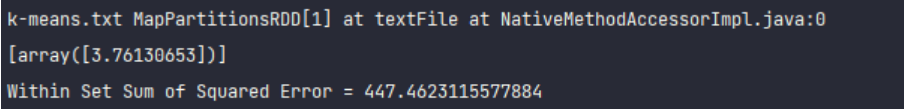
\includegraphics[width=0.9\textwidth]{images/1.png}  
\end{figure}   

如上图所示,当聚类为1个节点时,评分在3分以上,说明该剧的口碑不错;\\

$\bullet$ 当聚类节点为2时:
\begin{figure}[H]
    \centering
    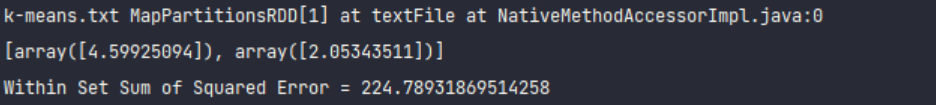
\includegraphics[width=0.9\textwidth]{images/2.png}  
\end{figure}   
该情况下,存在两个聚类点,且两个聚类点之间差距较大,说明该剧存在评论两极分化的情况;进一步,对评论星级5以及星级2,1的评论的可靠性进行分析,依然利用k-means算法进行计算;\\

$\bullet$ \textbf{低分评论可靠性聚类点:(1星,2星)}
\begin{figure}[H]
    \centering
    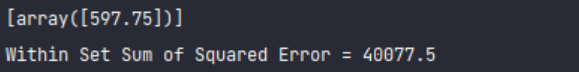
\includegraphics[width=0.8\textwidth]{images/3.png}  
\end{figure}  

$\bullet$ \textbf{高分评论可靠性聚类点:(4星,5星)}

\begin{figure}[H]
    \centering
    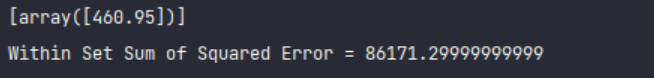
\includegraphics[width=0.8\textwidth]{images/4.png}  
\end{figure}  

\subsubsection{结果分析}
通过聚类结果,我们可以发现对该部电影的打分存在两极化现象,然而对其中高分和低分评论进行可靠性聚类,可以发现高分的可靠性要明显低于低分可靠性,而且高分评论的可靠性分数比较分散,并不集中,这从一定程度上说明该部电影的评论可能存在以下问题:\\

\begin{itemize}
    \item 可能存在少量刷评论水军;
    \item 可能存在电影给观众印象不深,导致评论出现偏颇现象;
\end{itemize}

\subsection{线性回归:国内外评分对比}
在上面的分析中,我们可以看到在豆瓣网上,对于电影《雄狮少年》的影评似乎存在一定问题。\\

豆瓣评分真的不够公平吗?评分高低真有这么大的影响吗?\\

为了找寻答案,我们采集了近5年国内院线电影的评分、票房等信息,尝试着用数据来解解惑。\\

\subsubsection{数据选取}
我们怀疑由于评分机制不合理、受到水军影响等原因,豆瓣评分很容易高估或者低估了一部电影,不能真正反映群众的观影评价。\\

我们找来了美国的主流电影评价网站IMDb与豆瓣进行对比,它们同采用十分制,也都来源于大众打分,存在较强的可比性。通过这次对比,来确定豆瓣的评价是否准确。\\

同一部电影在两家网站上的表现差异有多大呢?我们对近5年的1128部电影进行了分析。\\

\subsubsection{数据可视化}

\begin{figure}[H]
    \centering
    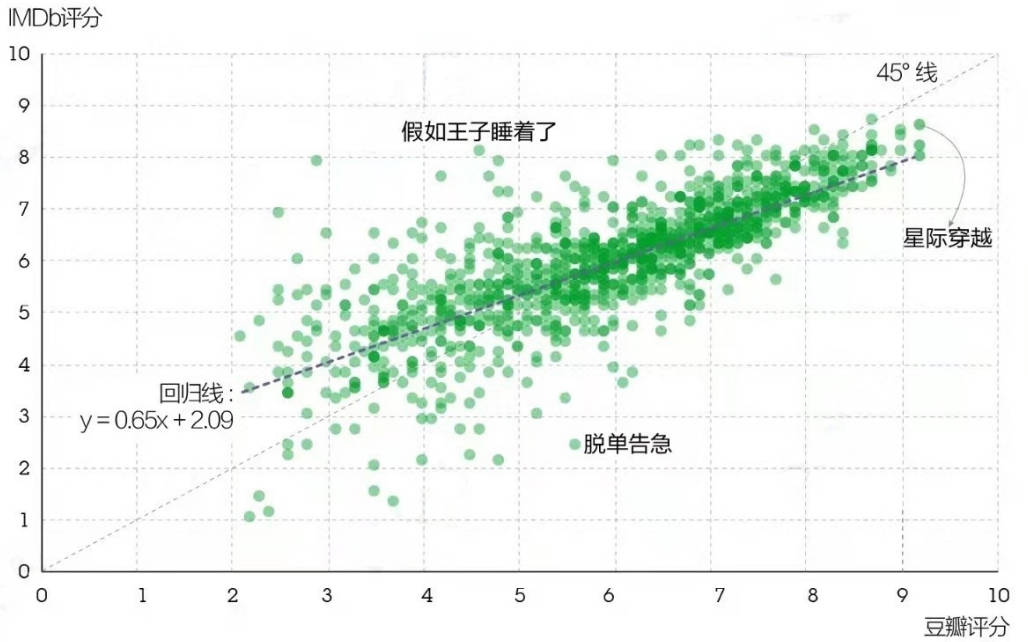
\includegraphics[width=0.9\textwidth]{images/douban-imdb.jpg}  
    \caption{近五年国内院线电影豆瓣与IMDb评分对比}
\end{figure}  

以豆瓣评分为横坐标,IMDb评分为纵坐标制图,每个圆点都代表一部电影,大致看去,豆瓣评分越高的电影,IMDb评分也越高。\\

我们进一步利用最小二乘法对两组数据进行了相关性检验,相关系数为0.65,说明同一部电影的豆瓣评分和IMDb评分存在65\%左右的高度相关。\\

我们查看了那些偏离回归线较远的电影点,发现在豆瓣和IMDb上表现差别最大的电影可以分为以下两大类:\\

$\bullet$ 拥有真爱粉或者真爱黑的烂片。比如一听名字就很有恋爱味道的《708090之深圳恋歌》,IMDb评分比豆瓣整整高出5分。

$\bullet$ 存在文化差异或者欣赏差异的电影。该类典型代表比如李安作品《比利·林恩的中场战事》,豆瓣评分8.4,IMDb评分却低至及格线。

而大多数电影,在两家网站上的表现比较一致。\\

\begin{figure}[H]  
\centering
 \begin{minipage}[t]{0.45\textwidth} 
  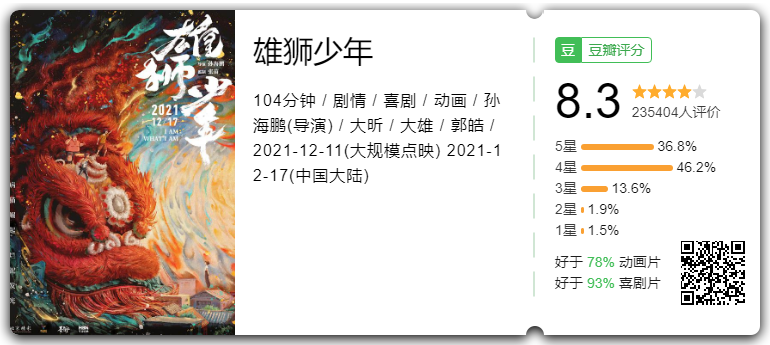
\includegraphics[scale = 0.25]{images/雄狮少年.png}
  \caption{《雄狮少年》豆瓣评分}
 \end{minipage}
 \begin{minipage}[t]{0.45\textwidth} 
  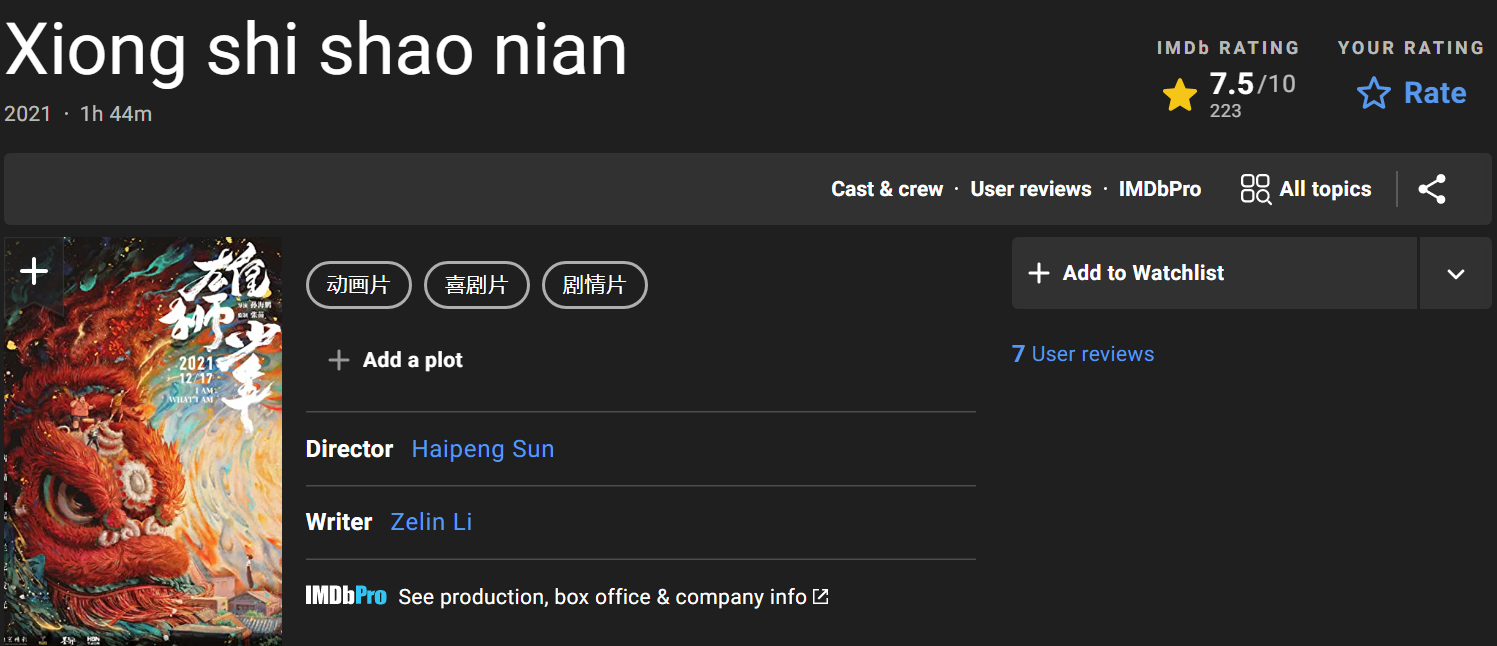
\includegraphics[scale = 0.15]{images/idmb-xssn.png}
  \caption{《雄狮少年》IMDb评分}
 \end{minipage}  
\end{figure}

豆瓣评分$x = 8.3$,和IMDb评分$\hat{y} = 7.5$,符合我们预测出两个网站评分之间的的线性回归方程$y = 0.65x + 2.09$,这说明在该电影在豆瓣上的评分并无较大问题。\\

\subsection{回归分析:票房与评分的关系}

考虑到影响电影票房的因素很多,除了影片的口碑和质量,还有知名度和关注量等。因此,我们在计算时,除了把电影豆瓣评分作为影片口碑的指代指标,并且加入了为该部电影评分的人数作为影响力的指代指标。\\

同时拥有票房和得分的有效数据共有1533组,为了所有变量在同一个数量级,我们在计算时电影票房以万元为单位,将其和豆瓣打分人数取自然对数。\\

假定关系是:
\begin{equation}
    In\mbox{(票房})= \mbox{系数1} \times \mbox{豆瓣评分} + \mbox{系数2}  \times In\mbox{(打分人数)} + \mbox{常数}C
\end{equation}


当我们用多元线性回归模型\footnote{样本量N = 1533, 利用OLS计算}对这些数据进行拟合之后,有了“惊人”的发现:精确度R2\footnote{模型精确程度用$R^{2}$表示,越趋近于1,代表模型越精确}说明豆瓣评分和打分人数可以在72.4\%的程度上解释电影的最终票房,并且三组参数\footnote{系数1是豆瓣评分前的系数,系数2是ln(打分人数)前的系数}都通过了假设检验,较为可信.\\

\begin{figure}[H]
    \centering
    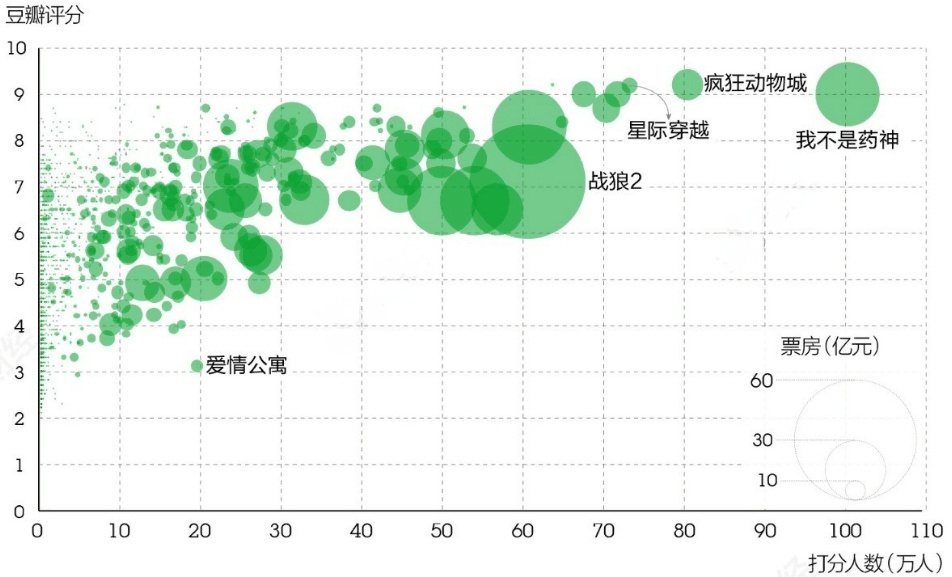
\includegraphics[width=0.9\textwidth]{images/打分-票房.jpg} 
    \caption{近五年国内院线电影豆瓣评分、评分人数与票房的关系}
\end{figure}  

\begin{table}[H]  
\begin{center}
\sffamily
\arrayrulecolor{white}
\arrayrulewidth=1pt
\renewcommand{\arraystretch}{1.5}
    \begin{tabular}{A||B|C|A|B} 
    \rowcolor{.!80!Black}
    \arraycolor{White}\bfseries 自变量 & 模型精确度($R^{2}$) &  系数1 & 系数2 & 常数C \\
    \hline
     \arraycolor{White}\bfseries 豆瓣评分,ln(评分人数) & 0.724 & -0.243 & 1.055 & -0.842 \\ 
     \hline
     \arraycolor{White}\bfseries 豆瓣评分 & 0.226 & 0.72 & & 3.2292 \\
     \hline  
     \arraycolor{White}\bfseries ln(评分人数) & 0.71 & & 0.936 & -1.08 \\
     \hline
    \end{tabular}
    \caption{模型精确度}
\end{center}
\end{table}  
 
 
我们分别对两个因素做回归分析,又有了新发现。\\

在单独分析时,豆瓣电影评分对于电影总票房有较为明显的正相关关系,并且还有22.6\%的精确度。而如果引入了热度数据,原本应该是正相关关系的豆瓣电影评分与电影总票房,却变为了负相关(尽管负得不明显)。\\

也就是说,热度对于票房的影响,显著大于豆瓣评分的作用。当然,一个电影的最终票房还会与包括宣发、排片、票补等多种因素有关,这些因素都会对结果产生干扰。但得承认一点,豆瓣评分高低和最终票房的关系,真的没有人气等其他因素作用那么大。\\

这说明通过攻击《雄狮少年》票房低来证明其是一部烂片,可能并不是十分严谨。\\


\subsection{Kmeans聚类II:如何识别被水军严重影响的电影?}
要想根据评分来正确判断一部电影的水准,最大的干扰项恐怕在于水军和黑子的涌入影响了大家对于评分的正常判断,那五星党/差评党会对电影评分造成多大程度的干扰呢? \\

\subsubsection{标准差定义}
我们在这里使用标准差作为衡量一部电影评分争议性的标准:\\
\begin{equation}
    S = \sqrt{Q} 
\end{equation}
\begin{equation}
    Q = P2(2-Avg)^{2}+P4(4-Avg)^{2}+...+P10(10-Avg)^{2}
\end{equation}
其中,S为标准差,Q为方差\\

$\bullet$对豆瓣星级按照1星对应2分,2星对应4分,5星对应10分的方式进行赋值

$\bullet$ Avg为该电影豆瓣得分

$\bullet$ P2、P4…P10为评分中1-5颗星所占的比例 \\

\subsubsection{数据可视化及分析}
根据每部电影的豆瓣评分与评分标准差,我们对1714部电影进行了聚类\footnote{样本量N=1714,按颜色分为7类},表现相似的电影在下图\footnote{纵坐标为评分标准差,指该电影再各个星段得分与最后总分的标准差,该值越大、点越高,代表这部电影的打分争议性更大}中属于同一颜色。\\

\begin{figure}[H]
    \centering
    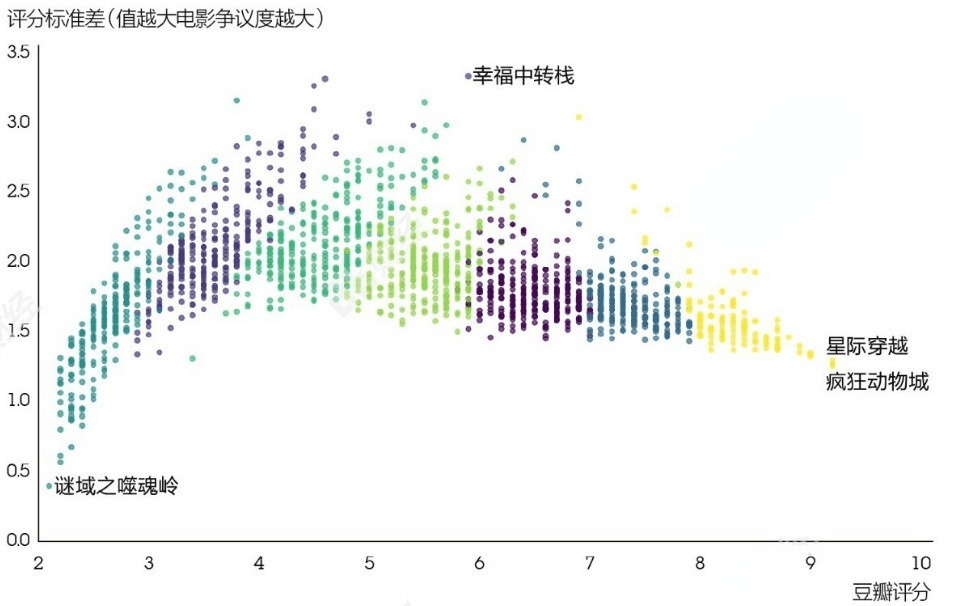
\includegraphics[width=0.9\textwidth]{images/评分标准差.jpg}
    \caption{近五年国内院线电影豆瓣口碑争议度聚类分析}
\end{figure}  

可以发现,低分电影和高分电影口碑分化都挺小,这意味着,对于绝对的好片与绝对的烂片,大家都没有太大争议。而中间段位的电影则是幺蛾子爆发区域,不管是由于水军/黑子/粉丝的影响,还是观众本身对这部电影就有较大的审美偏差,总之,这个分段的电影往往争议性较大,评分的普适参考性就小了些。\\

我们将电影《雄狮少年》的数据带入上式,得到的标准差S值为1.665,这说明该电影并不存在口碑分化。
 


\section{结论}
\subsection{公众情绪与时效性}
当网络上出现某一热点时间,往往会非常迅速地形成一种情绪化的意见。在这部电影上映初期,对于这部电影的评价几乎全为负面。随着时间的流逝,越来越多的人观看了这部电影,这对后续的舆情有较大的影响,客观中立的意见变得越来越多了。\\

尽管如此,对于这部电影,负面评价压倒了正面评价,从LDA主题以及词云图,我们也可得知,在初印象上,这部电影似乎并不讨观众喜欢。

\subsection{涉嫌辱华}
我们可以通过数据可视化直观地看到多数网友均认为影片中的人物形象涉嫌辱华,尤其是剧中人物的眯眯眼有崇洋媚外。这激起了公众情绪,让这部电影的电影陷入了十分不利的地步。

\subsection{优秀动漫}
通过分析豆瓣影评我们可以知道,该动漫没有陷入对日美漫画的模仿、并且结合了中国传统的舞狮文化,是一部优秀的动漫。

\subsubsection{当前网络环境难以达成共识}
在同一平台上存在着激烈的争论,这证明了当前网络环境复杂多变,人们难以对公共事件打成一致看法

\subsubsection{舆论主体身份}
大数据时代,随着网络的普及和新媒体的应用,越来越多的公众断则到网络上发言。舆论主体从传统媒介转变为网络媒介及公共民众。

\subsection{不同平台具有不同的用户画像}
我们通过大量来自豆瓣的数据分析,可得该电影并不存在明显口碑分化,也不存在明显的网络水军现象。\\

但是, 知乎网站和bilibili弹幕网所得到的分析均显示网友们对其是负面评价。\\

即,不同平台拥有不同的用户,用户人群画像不同,自然很可能对同一事物产生不同的评价.\\

\subsection{网络回声室}

另一个可能推测是:这可能与网络回声室\footnote{\noindent 
\textbf{“回声室效应”}:指在一个网络空间里,如果你听到的都是对你意见的相类回响,你会认为自己的看法代表主流,从而扭曲你对一般共识的认识。}现象有关。 \\

具体表现就是,在知乎对该电影呈现负面评价的人不会到豆瓣网上给该电影打低分。在豆瓣上给该电影高分的人,看到其他网站都是对该电影的负面评价,可能就选择不发言了。\\

这说明该电影在艺术上具有一定优秀之处,但在一些具体的处理上,没有照顾好公众情绪。




\newpage
\begin{subappendices}  
\section{附录:小组分工} 

\subsection{王红阳}
\begin{itemize}
    \item 编写爬虫,爬取知乎回答,豆瓣影评及bilibili视频评论
    \item '数据采集'报告书写
    \item 词云图代码编写
    \item TF-IDF,LDA代码编写及报告书写
    \item ‘结论’报告书写
\end{itemize}

\subsection{夏睿}
\begin{itemize}
    \item '背景及意义'报告书写
    \item 爬取bilibili弹幕
    \item K-means聚类代码编写
    \item ‘K-means聚类'报告书写
\end{itemize}

\subsection{窦浩阳}
\begin{itemize}
    \item '技术路线'文档书写
    \item word-count代码编写
    \item 线性回归代码编写
    \item ‘线性回归’文档书写
\end{itemize}

\subsection{周浩然}
\begin{itemize}
    \item 百家号,知网数据抓取
    \item 数据清洗
    \item 情感分析代码编写
    \item ‘情感分析’报告书写
\end{itemize}

\end{subappendices}  % 附录内容结束

\end{document}